\chapter{Background}

Lew Platt once commented in the 1980s: ``If only HP (Hewlett-Packard\footnote{https://www.hp.com}) knew what HP  knows, we would be three times more productive.'' His words indicate that the problem of fully utilizing all expertise within an organization is desirable but hard to achieve for organizations (especially as large as HP). For a software development organization, failing to identify and select proper expertise is a threat which lowers productivity, and further overburden central individuals (\textit{expertise escalation}), e.g., core product manager, in the organization \cite{mcdonald1998just}. As the development of information technology, software engineering is vital for human beings' daily activities, and the failure of software may further threat the quality of our lives and may lead to hazard at the society level. Locating and then utilizing an organization's own \textit{intangible human resources} is a challenging two-step (location and utilization) process for all software organizations and communities \cite{bohlander2010managing}. Extracting specific domain expertise from individual talent among these organizations is the critical first step.

\section{Nature of Expertise and Expert}

To locate expertise precisely, first, we need to have a clear understanding of the nature of expertise and who have them. According to the view of a psychologist, \citeauthor{ericsson2006cambridge} define expertise as the ``\textit{characteristics, skills and knowledge}'' in a relative approach while comparing experts to novices and less experienced people \cite{ericsson2006cambridge}. Their definition illustrates that people with related expertise would have better performance than those without it.

\begin{displayquote}
``\textit{Expert: one who is very skillful and well-informed in some special field.}'' -Webster's New World Dictionary

``\textit{Experts are people who produce clearly above average (outstanding) performance on a regular basis.}'' -Cambridge handbook of Expertise and Expert Performance
\end{displayquote}

The above two definitions of expert are from Webster's New World Dictionary \cite{guralnik1983webster}, and Cambridge handbook of Expertise and Expert Performance \cite{ericsson2006cambridge} respectively. Both of them suggest a relative approach to define expert by comparing experts performance with novices. However, as previous research suggests, there is another approach to identify experts by studying genuinely exceptional people, with the goal of understanding how they perform \cite{chi2006two}.

In addition to \citeauthor{ericsson2006cambridge}'s view, from a neuroscience perspective in \citeauthor{bilalić2017neuroscience}'s research on explaining the nature of expertise \cite{bilalić2017neuroscience}, \citeauthor{bilalić2017neuroscience} classifies the expertise into categories. There are three major types of expertise when human beings are referring to the skills and specialties that expert masters:

\begin{itemize}
\item \textit{Perceptual Expertise}: This type of expertise that predominantly rely on the information directly come from human biological senses. For instance, the radiologist example mentioned in \citeauthor{bilalić2017neuroscience} mentioned, who could enable her visual expertise while detecting the problem of the patient through an X-ray photo.
\item \textit{Cognitive Expertise}: The second type of expertise focuses on the memory engagement and mental stimulation, rather than information gathering process in the perceptual expertise, such as mathematical calculation skills. Particularly, the state-of-the-art research on software engineering expertise (for example, \cite{Anvik2006who, mcdonald2000expertise, mockus2002expertise, fritz2010degree, yu2016reviewer, costa2016tipmerge}) focuses on this type of expertise when looking for programming experts.
\item \textit{Motor Expertise}: the last type of expertise is the muscle and body control ability, such as dancing, sports, playing music and other general movements. An example expert of this type could be a professional basketball player who can hit shots from long range in a higher chance than an ordinary novice.
\end{itemize}

In addition, if we look at a definition of expertise by software engineering researcher by \citeauthor{mockus2002expertise} \cite{mockus2002expertise}: 

\begin{displayquote}
``Expertise is defined as the skill of an expert, and, if interpreted quantitatively, reflects the degree of the ability of a person to perform a certain task.''
\end{displayquote}

The concept of expertise can be interpreted as a quantitative value, but in reality, it is very complicated to measure, for example, early studies in cognitive science use eyeball tracking to determine the information processing ability which is an indicator of expertise \cite{gobet1996recall}.

Another general expectation of experts is that they could utilize their expertise and previous experience to handle any unexpected situation and outcome \cite{ericsson2006cambridge}. Since experts have already acquired enough knowledge as a structured system in their \textit{long-term memory}, they would quickly adopt the situation in their field, and they also would be able to automatically provide and recognize reasonable solutions rather than figure them out.

In this study, we would cover basic approaches to locating expertise (absolute and relative), comparing their measurement of expertise, and finally evaluate these expertise location studies. Moreover, we attempt to summarize literature that considers the above two factors, i.e., memory recalling procedure, and evaluating expertise location methods.

\section{Memory Engagement and Expertise}

As this study particularly focuses the expertise and expert location in the field of programming and software engineering, the most critical type of expertise is the \textit{cognitive expertise}, though the other two types could also be involved in the software production. The connection between memory and expertise is very tight due to our memory storage system. Many studies have been conducted on the structural model of human memory, and memory/expertise retrieval mechanism. The most related ones are the \textit{Chess Experiment} for \textit{Chunking theories} \cite{chase1973perception, de2008thought, gobet1996recall} and the \textit{Amnesia Patient Experiment} \cite{cohen1980preserved}.

\begin{figure}
\includegraphics[width = 1\columnwidth]{memory_store.png}
\centering
\caption{The different memory sections, and the process of transferring and retrieving relation between sensory store, short-term memory and long-term memory}
\label{memoryStore}
\end{figure}

Human beings receive raw information and store it at the sensory store, but only if the information got human attention, the information would be processed to the \textit{short-term memory}, which is not everlasting and typical only stay for about 18 seconds without rehearsal \cite{revlin2012cognition}. Further, through several iterations of rehearsal, information in short-term memory would be transferred to \textit{Long-term Memory} which is the \textit{Synaptic Consolidation} process \cite{dudai2004memory}, and the information is hard to forget through a forgetting process. Therefore, the long-term memory reflection is an essential indicator of having the expertise, and cognitive literature has also supported it. 

\begin{displayquote}
Hence we can say that one part of the grand-master's chess skill resides in the 50,000 chunks stored in memory, and in the index (in the form of a structure of feature tests) that allows him to recognize any one of these chunks on the chess board and to access the information in long-term memory that is associated with it. The information associated with familiar patterns may include knowledge about what to do when the pattern is encountered. Thus the experienced chess player who recognizes the feature called an open file thinks immediately of the possibility of moving a rook to that file. The move may or may not be the best one, but it is one that should be considered whenever an open file is present. The expert recognizes not only the situation in which he finds himself but also what action might be appropriate for dealing with it.
\end{displayquote}

As mention by Simon in his masterpiece, the Science of the Artificial \cite{Simon:1996:SA:237774}, when referring to experts, we expected that they could retrieve their similar experience or expertise to solve the problem at hand, and De Groot lead studies on the expertise retrieval from long-term memory and purposed the chunking theory \cite{chase1973perception, de2008thought, gobet1996recall}. Early in 1965, De Groot conducted the chess experiment to explore the performance difference between chess experts and novices by recalling chess positions. Each participant would have 5 seconds of viewing and remember the chess board with positioned pieces and then trying to re-position all pieces on the board. However, in short, experienced expert chess players could recall more pieces and make fewer mistakes. As the progress made in neurobiology, researchers realize that information is stored in memory as chunks \cite{chase1973perception}. Chase and Simon in their following study of chess experiment, they explain the superior performance of experts with the better functioning ability of chunks. Experts could retrieve more and larger chunks from their memory of specialized field. In addition, a later study \cite{richman1995simulation} suggests that once experts encounter a new/unexpected situation in their specific domain, and then experts would automatically active their domain-specific expertise in long-term memory, which supports the second expectation for an expert in section 2.1.

\usetikzlibrary{trees}

\begin{figure}
\centering
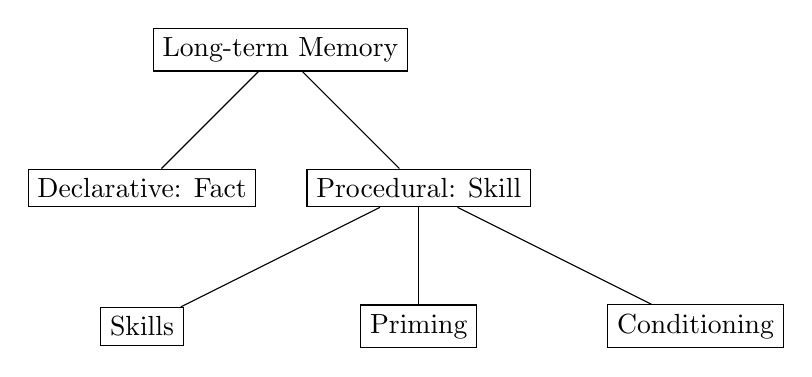
\begin{tikzpicture}[sibling distance=10em, level distance = 5em,
  every node/.style = {shape=rectangle,
    draw, align=center}]]
  \node {Long-term Memory}
    child { node {Declarative: Fact} }
    child { node {Procedural: Skill}
        child { node {Skills} }
        child { node {Priming} }
        child { node {Conditioning} } };
\end{tikzpicture}
\caption{Knowing that (declarative) vs. Knowing how (procedural): the long-term memory model from \citeauthor{cohen1980preserved} \cite{cohen1980preserved}}
\label{LTM model}
\end{figure}

Further, it is worth noticing that, according to empirical results, there is a difference between ``knowing what'' and ``knowing how'' in human long-term memory. In 1980, Cohen and Squire conducted the study on Amnesia patients to the exam which part of patient memory or totally had been impaired \cite{cohen1980preserved}. However, the result suggested a structural model of long-term memory which is detached. The performance of patients suggests that Amnesia patients' ``knowing what'' ability is impaired, but their ability to acquire or recall (``knowing how'') skills still remain. For example, they could learn or recall how to ride a bicycle. Their study creates an initial structural model for long-term memory, and our study would refer to this series of models to analyze long-term memory reflection from surveyed literature.

\section{Expertise Location in Software Engineering}

Chunking theory can also explain the developer performance in software products based on empirical results. \citeauthor{MCKEITHEN1981307} have conducted a study on the performance difference between programming novices and experts \cite{MCKEITHEN1981307}, and it empirically confirmed that experts have superior performance throughout experiments, and also they confirmed that chunk theory still holds for programming performance, as experts can recall more programming concepts while solving the problems. In addition to information processing ability, \citeauthor{MCKEITHEN1981307} also mentioned that the organization of computer programming knowledge in experts mind are remarkably similar, but not identical. However, following up studies on expert performance fail to utilize expert similarity to locate experts.

A software system is an artifact that requires tremendous effort to develop due to its complex nature, and there is no one for all solution to increase software productivity \cite{brooks1987no}. Due to the complexity of software engineering, there are many sub-domains of expertise. Moreover, OSS libraries are increasingly used as components in other software artifacts. Hence, identification of the specific domain experts is particularly hard in the context of freely formed OSS teams.

\begin{figure}
\includegraphics[width = 0.8\columnwidth]{radiologist}
\centering
\caption{The Radiologist Example That \citeauthor{bilalić2017neuroscience} Uses in \cite{bilalić2017neuroscience} Which Shows the Difference Between Experts and Novices When Processing Information}
\label{radiologist}
\end{figure}

It is a long-discussed question to define and measure expertise in a quantitative approach systematically. A quantitative approach to measure the expertise level of chess players is tracking their eyeball movement, since expert has the ability to automatically exclude irrelevant information, i.e., chess master has the capacity to focus on the most critical part of board for winning the game, but novice is not able to focus on the relevant part for planning winning strategy. Similarly, expert radiologist only needs a few glances to understand an X-ray with very few eye focus movement, but novices like medical students require more time and effort for the same process \citep{bilalić2017neuroscience}. There are several pioneer studies for locating experts in software developing process \cite{mcdonald1998just, mcdonald2000expertise, mockus2002expertise, Reichling2007}. As \citeauthor{mcdonald2000expertise} found in their studies \cite{mcdonald1998just, mcdonald2000expertise}, one of the most effective way in engineering practice identifies expert according to developer's previous experience, which could be reflected by two indicators: a developer's historical artifacts, and people whom she has worked with (her professional social network). Their work has been followed up by other researchers in software engineering, and most of their work focuses on extracting the higher precise and accurate expertise identification over historical artifacts such as code \cite{ Anvik2006who, mockus2002expertise, Servant2011history}.

Nevertheless, these expertise identification systems are considered biased due to only enabling public information, and user reputation could be easily manipulated by faking data or operating multiple accounts. However, data provided through these user-generated content enables more data sources than previous methods, and as the open source software is increasingly involved in other software engineering process, either in academia or commercial industry. The transparency provided by OSS collaboration sites could afford more activity information while locating expertise \cite{Dabbish2012social}, and distributed collaboration approach also benefit from an automated expertise identification when the team is not familiar with each other. On the other hand, precisely locating the best knowledge providers on knowledge sharing can also smooth the process with a better result.

However, in addition to mining historical artifacts, there is emerging emphasis on social networking functions for online software collaboration sites \cite{Dabbish2012social} and Q\&A knowledge sharing sites \cite{vasilescu2014social}. To encourage participant and reward contributors, these platforms provide endorsements, ratings, stars, reputation point, and other rewarding systems to acknowledge the achievement of a software developer through certification provided by her peers who use the same platform, or records in the system. 

There are a few studies \cite{hiring2016sarma} that enable these various data generated by other users. The results have suggested it is promising in hiring software developer occupations even though interviews are necessary. We will present our detailed survey results in the chapter 4.